% GNUPLOT: LaTeX picture with Postscript
\begingroup
\newcommand{\ft}[0]{\footnotesize}\newcommand{\ty}[0]{\tiny}
  \makeatletter
  \providecommand\color[2][]{%
    \GenericError{(gnuplot) \space\space\space\@spaces}{%
      Package color not loaded in conjunction with
      terminal option `colourtext'%
    }{See the gnuplot documentation for explanation.%
    }{Either use 'blacktext' in gnuplot or load the package
      color.sty in LaTeX.}%
    \renewcommand\color[2][]{}%
  }%
  \providecommand\includegraphics[2][]{%
    \GenericError{(gnuplot) \space\space\space\@spaces}{%
      Package graphicx or graphics not loaded%
    }{See the gnuplot documentation for explanation.%
    }{The gnuplot epslatex terminal needs graphicx.sty or graphics.sty.}%
    \renewcommand\includegraphics[2][]{}%
  }%
  \providecommand\rotatebox[2]{#2}%
  \@ifundefined{ifGPcolor}{%
    \newif\ifGPcolor
    \GPcolortrue
  }{}%
  \@ifundefined{ifGPblacktext}{%
    \newif\ifGPblacktext
    \GPblacktextfalse
  }{}%
  % define a \g@addto@macro without @ in the name:
  \let\gplgaddtomacro\g@addto@macro
  % define empty templates for all commands taking text:
  \gdef\gplbacktext{}%
  \gdef\gplfronttext{}%
  \makeatother
  \ifGPblacktext
    % no textcolor at all
    \def\colorrgb#1{}%
    \def\colorgray#1{}%
  \else
    % gray or color?
    \ifGPcolor
      \def\colorrgb#1{\color[rgb]{#1}}%
      \def\colorgray#1{\color[gray]{#1}}%
      \expandafter\def\csname LTw\endcsname{\color{white}}%
      \expandafter\def\csname LTb\endcsname{\color{black}}%
      \expandafter\def\csname LTa\endcsname{\color{black}}%
      \expandafter\def\csname LT0\endcsname{\color[rgb]{1,0,0}}%
      \expandafter\def\csname LT1\endcsname{\color[rgb]{0,1,0}}%
      \expandafter\def\csname LT2\endcsname{\color[rgb]{0,0,1}}%
      \expandafter\def\csname LT3\endcsname{\color[rgb]{1,0,1}}%
      \expandafter\def\csname LT4\endcsname{\color[rgb]{0,1,1}}%
      \expandafter\def\csname LT5\endcsname{\color[rgb]{1,1,0}}%
      \expandafter\def\csname LT6\endcsname{\color[rgb]{0,0,0}}%
      \expandafter\def\csname LT7\endcsname{\color[rgb]{1,0.3,0}}%
      \expandafter\def\csname LT8\endcsname{\color[rgb]{0.5,0.5,0.5}}%
    \else
      % gray
      \def\colorrgb#1{\color{black}}%
      \def\colorgray#1{\color[gray]{#1}}%
      \expandafter\def\csname LTw\endcsname{\color{white}}%
      \expandafter\def\csname LTb\endcsname{\color{black}}%
      \expandafter\def\csname LTa\endcsname{\color{black}}%
      \expandafter\def\csname LT0\endcsname{\color{black}}%
      \expandafter\def\csname LT1\endcsname{\color{black}}%
      \expandafter\def\csname LT2\endcsname{\color{black}}%
      \expandafter\def\csname LT3\endcsname{\color{black}}%
      \expandafter\def\csname LT4\endcsname{\color{black}}%
      \expandafter\def\csname LT5\endcsname{\color{black}}%
      \expandafter\def\csname LT6\endcsname{\color{black}}%
      \expandafter\def\csname LT7\endcsname{\color{black}}%
      \expandafter\def\csname LT8\endcsname{\color{black}}%
    \fi
  \fi
    \setlength{\unitlength}{0.0500bp}%
    \ifx\gptboxheight\undefined%
      \newlength{\gptboxheight}%
      \newlength{\gptboxwidth}%
      \newsavebox{\gptboxtext}%
    \fi%
    \setlength{\fboxrule}{0.5pt}%
    \setlength{\fboxsep}{1pt}%
\begin{picture}(3888.00,3600.00)%
    \gplgaddtomacro\gplbacktext{%
      \csname LTb\endcsname%
      \put(528,638){\makebox(0,0)[r]{\strut{}\ft 0.1}}%
      \csname LTb\endcsname%
      \put(528,1207){\makebox(0,0)[r]{\strut{}\ft 1}}%
      \csname LTb\endcsname%
      \put(528,1777){\makebox(0,0)[r]{\strut{}\ft 10}}%
      \csname LTb\endcsname%
      \put(528,2346){\makebox(0,0)[r]{\strut{}\ft 100}}%
      \csname LTb\endcsname%
      \put(528,2915){\makebox(0,0)[r]{\strut{}\ft 1000}}%
      \put(3491,418){\makebox(0,0){\strut{}$\infty$}}%
      \put(660,418){\makebox(0,0){\strut{}\ft 1}}%
      \put(943,418){\makebox(0,0){\strut{}\ft 2}}%
      \put(1226,418){\makebox(0,0){\strut{}\ft 3}}%
      \put(1509,418){\makebox(0,0){\strut{}\ft 4}}%
      \put(1792,418){\makebox(0,0){\strut{}\ft 5}}%
      \put(2076,418){\makebox(0,0){\strut{}\ft 6}}%
      \put(2359,418){\makebox(0,0){\strut{}\ft 7}}%
      \put(2642,418){\makebox(0,0){\strut{}\ft 8}}%
      \put(2925,418){\makebox(0,0){\strut{}\ft 9}}%
      \put(3208,418){\makebox(0,0){\strut{}\ft 10}}%
    }%
    \gplgaddtomacro\gplfronttext{%
      \csname LTb\endcsname%
      \put(-44,1776){\rotatebox{-270}{\makebox(0,0){\strut{}\ft Port queue lengths in flits}}}%
      \put(2075,154){\makebox(0,0){\strut{}\ft Maximum port queue size}}%
      \csname LTb\endcsname%
      \put(1508,3467){\makebox(0,0)[r]{\strut{}\ty IDA-UC max}}%
      \csname LTb\endcsname%
      \put(1508,3327){\makebox(0,0)[r]{\strut{}\ty G2C3 max}}%
      \csname LTb\endcsname%
      \put(1508,3187){\makebox(0,0)[r]{\strut{}\ty G2C4 max}}%
      \csname LTb\endcsname%
      \put(2579,3467){\makebox(0,0)[r]{\strut{}\ty avg}}%
      \csname LTb\endcsname%
      \put(2579,3327){\makebox(0,0)[r]{\strut{}\ty avg}}%
      \csname LTb\endcsname%
      \put(2579,3187){\makebox(0,0)[r]{\strut{}\ty avg}}%
    }%
    \gplbacktext
    \put(0,0){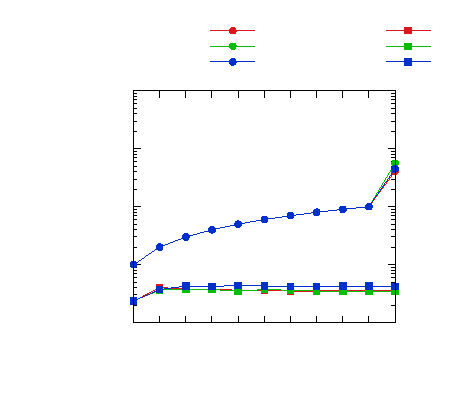
\includegraphics{../plots/queuelengths-ports}}%
    \gplfronttext
  \end{picture}%
\endgroup
